% Authors: Taejin Hwang
% Emails: taejin@berkeley.edu

\qns{System Identification}

In this question, we will take a look at how to \textbf{identify} a system by taking experimental data taken from a (presumably) linear system to learn a discrete-time linear model for it using the least-squares.

Recall that a \textbf{linear, continuous-time,} system can be put in state-space form:
\begin{equation}
\ddt{}{t} \vec{x}(t) = A \vec{x}(t) + \vec{b} u(t)
\end{equation}

Now let's say we have an \textbf{unknown} linear system in which we can give an input $u(t)$ and observe the output $\vec{x}(t).$ We can model the system using the following diagram:
\begin{center}
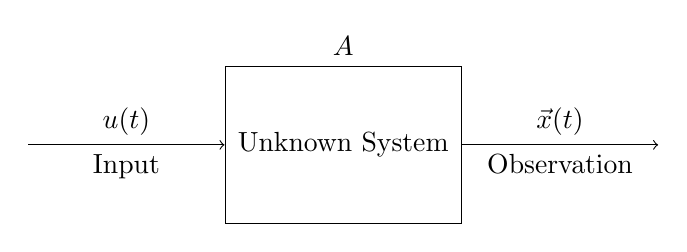
\begin{tikzpicture}
\node[draw, rectangle, minimum width = 3 cm, minimum height = 2 cm] (fl) at (0,0) {Unknown System};
\node[above] at (fl.north) {$A$};
\draw[<-] (fl) -- node[above]{$u(t)$} node[below]{Input} ++(-4,0);
\draw[->] (fl) -- node[above]{$\vec{x}(t)$} node[below]{Observation} ++(4,0);
\end{tikzpicture}
\end{center}

Recall from discussion that if we put a \textbf{piecewise constant} input $u(t) = u(i)$ for $t \in [i, i+1),$ then we can observe the output $\vec{x}(t)$ at time $t = i + 1,$ and form a discretized model of the observation. 

\begin{center}
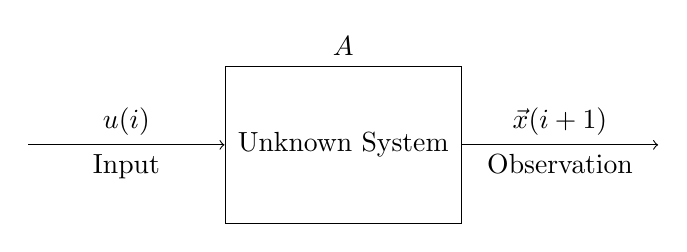
\begin{tikzpicture}
\node[draw, rectangle, minimum width = 3 cm, minimum height = 2 cm] (fl) at (0,0) {Unknown System};
\node[above] at (fl.north) {$A$};
\draw[<-] (fl) -- node[above]{$u(i)$} node[below]{Input} ++(-4,0);
\draw[->] (fl) -- node[above]{$\vec{x}(i + 1)$} node[below]{Observation} ++(4,0);
\end{tikzpicture}
\end{center}

\textbf{If} we knew the system, the relationship between $\vec{x}(i+1), \vec{x}(i),$ and $u(i)$ would be:
\begin{equation}
\vec{x}(i + 1) = A \vec{x}(i) + \vec{b} u(i)
\end{equation}

While this relation is useful, we currently do not know what the $A$ matrix or $\vec{b}$ vector are.

Therefore, we will start by creating unknown variables for the $A$ matrix, and $\vec{b}$ vector:
\begin{equation}
A = \begin{bmatrix} a_{11} & a_{12} \\ a_{21} & a_{22} \end{bmatrix} \ \ \text{and} \ \ \vec{b} = \begin{bmatrix} b_{1} \\ b_{2} \end{bmatrix}
\end{equation}
For the purposes of this question, we will be in the space $\mathbb{R}^2.$

\begin{enumerate}
  \qitem Let's say the system initially started at $\vec{x}(0) = \begin{bmatrix} x_{1}(0) \\ x_{2}(0) \end{bmatrix},$ and we gave an input at time $t = 0, \ u(0).$ 
  At time $t = 1,$ we observe $\vec{x}(1) = \begin{bmatrix} x_{1}(1) \\ x_{2}(1) \end{bmatrix}.$
  \textbf{How can you uncouple this matrix/vector equation into a system of linear equations?}

  \sol {
    We start by writing out the matrix/vector equation for our unknown system:
    \begin{equation}
    \vec{x}(1) = \begin{bmatrix} x_{1}(1) \\ x_{2}(1) \end{bmatrix} = A \vec{x}(0) + \vec{b} u(0) = 
    \begin{bmatrix} a_{11} & a_{12} \\ a_{21} & a_{22} \end{bmatrix} \begin{bmatrix} x_{1}(0) \\ x_{2}(0) \end{bmatrix} + 
    \begin{bmatrix} b_{1} \\ b_{2} \end{bmatrix} u(0)
    \end{equation}

    Uncoupling these equations, we get:
    \pagebreak[0]
    \begin{gather*}
    x_{1}(1) = a_{11} x_{1}(0) + a_{12} x_{2}(0) + b_{1} u(0) \\
    x_{2}(1) = a_{21} x_{1}(0) + a_{22} x_{2}(0) + b_{2} u(0)
    \end{gather*}
  }

  \qitem Based on the system of linear equations created in the previous part, \textbf{how many unknown} variables do we have? Also, if we have a system of linear equations with $n$ unknown variables, at the minimum, \textbf{how many equations} would we need to solve our system?

  \sol {
    The unknowns in this system of linear equations are: $a_{11}, a_{12}, a_{21}, a_{22}, b_{1}, b_{2}.$ \vskip 1pt
    If we have a system of linear equations with $n$ unknown variables, we will need at least $n$ equations to solve the system. 
  }

  \qitem We now give another input at $t = 1, \ u(1),$ and observe $\vec{x}(2).$ \vskip 1pt 
  \textbf{How many more equations do we get from this observation?}
  Also, how many more inputs will we need to observe until we have enough equations?

  \sol {
    We can write out a similar observation as the one made in part(a):
    \begin{equation}
    \vec{x}(2) = \begin{bmatrix} x_{1}(2) \\ x_{2}(2) \end{bmatrix} = A \vec{x}(1) + \vec{b} u(1) = 
    \begin{bmatrix} a_{11} & a_{12} \\ a_{21} & a_{22} \end{bmatrix} \begin{bmatrix} x_{1}(1) \\ x_{2}(1) \end{bmatrix} + 
    \begin{bmatrix} b_{1} \\ b_{2} \end{bmatrix} u(1)
    \end{equation}

    Uncoupling these equations again, we will get:
    \pagebreak[0]
    \begin{gather*}
    x_{1}(2) = a_{11} x_{1}(1) + a_{12} x_{2}(1) + b_{1} u(1) \\
    x_{2}(2) = a_{21} x_{1}(1) + a_{22} x_{2}(1) + b_{2} u(1)
    \end{gather*}
    Notice that for every observation we make at a given time step, we will get $2$ more equations. 
    This means we will have to look at a total of $3$ time steps to get $6$ equations.
    Taking the initial condition $\vec{x}(0)$ into account, we will have to observe a total of $4$ inputs.
  }

  \qitem Assuming we have taken all of the necessary measurements of $x(t)$ at time $t = 0, 1, 2, ...$ \vskip 1pt
  \textbf{How can we set up our system of linear equations as a matrix-vector equation?}

  \sol {
    We can set up the following system of linear equations:
    $$
    \begin{bmatrix}
    x_{1}(0) & x_{2}(0) & u(0) & 0 & 0 & 0 \\
    x_{1}(1) & x_{2}(1) & u(1) & 0 & 0 & 0 \\
    x_{1}(2) & x_{2}(2) & u(2) & 0 & 0 & 0 \\
    0 & 0 & 0 & x_{1}(0) & x_{2}(0) & u(0) \\
    0 & 0 & 0 & x_{1}(1) & x_{2}(1) & u(1) \\
    0 & 0 & 0 & x_{1}(2) & x_{2}(2) & u(2) 
    \end{bmatrix} 
    \begin{bmatrix} a_{11} \\ a_{12} \\ b_{1} \\ a_{21} \\ a_{22} \\ b_{2} \end{bmatrix}
    = \begin{bmatrix} x_{1}(1) \\ x_{1}(2) \\ x_{1}(3) \\ x_{2}(1) \\ x_{2}(2) \\ x_{2}(3) \end{bmatrix}$$
    This can be written in as a matrix vector equation $D \vec{s} = \vec{y}$ and we can solve for $\vec{s} = D^{-1} \vec{y}$  
  }

  \qitem While we can set up a matrix vector equation and uniquely solve our system, the output of the system can be noisy.
  Therefore, we update our model by considering a noise term $w(i)$ at time $t = i.$
  \begin{equation}
    \vec{x}(i + 1) = A \vec{x}(i) + \vec{b} u(i) + w(i)
  \end{equation}
  How can we set up a system of equations in a similar fashion but with a noise vector $\vec{w}?$
  \begin{equation}
    \vec{y} = D \vec{s} + \vec{w}
  \end{equation}

  \sol {
    $$
    \begin{bmatrix} x_{1}(1) \\ x_{1}(2) \\ x_{1}(3) \\ x_{2}(1) \\ x_{2}(2) \\ x_{2}(3) \end{bmatrix} 
    = 
    \begin{bmatrix}
    x_{1}(0) & x_{2}(0) & u(0) & 0 & 0 & 0 \\
    x_{1}(1) & x_{2}(1) & u(1) & 0 & 0 & 0 \\
    x_{1}(2) & x_{2}(2) & u(2) & 0 & 0 & 0 \\
    0 & 0 & 0 & x_{1}(0) & x_{2}(0) & u(0) \\
    0 & 0 & 0 & x_{1}(1) & x_{2}(1) & u(1) \\
    0 & 0 & 0 & x_{1}(2) & x_{2}(2) & u(2) 
    \end{bmatrix} 
    \begin{bmatrix} a_{11} \\ a_{12} \\ b_{1} \\ a_{21} \\ a_{22} \\ b_{2} \end{bmatrix}
    + \begin{bmatrix} w(0) \\ w(1) \\ w(2) \\ w(0) \\ w(1) \\ w(2) \end{bmatrix} $$
  }

  \qitem We can try to solve our system of equations, but we do not know what $\vec{w}$ is. \vskip 1pt
  What we can do however, is to take more measurements, and set up a \textbf{least squares} problem as seen in 16A.
  What would the least squares problem be if we took measurements up to time step $t = 5?$ 

  \sol {
  $$
    \begin{bmatrix} x_{1}(1) \\ x_{1}(2) \\ x_{1}(3) \\ x_{1}(4) \\ x_{1}(5) \\ x_{2}(1) \\ x_{2}(2) \\ x_{2}(3) \\ x_{2}(4) \\ x_{2}(5) \end{bmatrix} 
    = 
    \begin{bmatrix}
    x_{1}(0) & x_{2}(0) & u(0) & 0 & 0 & 0 \\
    x_{1}(1) & x_{2}(1) & u(1) & 0 & 0 & 0 \\
    x_{1}(2) & x_{2}(2) & u(2) & 0 & 0 & 0 \\
    x_{1}(3) & x_{2}(3) & u(3) & 0 & 0 & 0 \\
    x_{1}(4) & x_{2}(3) & u(4) & 0 & 0 & 0 \\
    0 & 0 & 0 & x_{1}(0) & x_{2}(0) & u(0) \\
    0 & 0 & 0 & x_{1}(1) & x_{2}(1) & u(1) \\
    0 & 0 & 0 & x_{1}(2) & x_{2}(2) & u(2) \\
    0 & 0 & 0 & x_{1}(3) & x_{2}(3) & u(3) \\
    0 & 0 & 0 & x_{1}(4) & x_{2}(4) & u(4) 
    \end{bmatrix} 
    \begin{bmatrix} a_{11} \\ a_{12} \\ b_{1} \\ a_{21} \\ a_{22} \\ b_{2} \end{bmatrix}
    + \begin{bmatrix} w(0) \\ w(1) \\ w(2) \\ w(0) \\ w(1) \\ w(2) \end{bmatrix} $$

    Which can equivalently be written as:
    \begin{equation}
      \vec{y} = D \vec{s} + \vec{w}
    \end{equation}
    For the least squares problem, we will want to minimize $\norm{\vec{w}}_{2} = \norm{y - D \vec{s}}_{2}$
    }

  \qitem How would we solve this least squares problem?

  \sol {
    Recall from 16A that if we are given the least squares problem:
    \begin{equation}
      A \vec{x} = \vec{b} + \vec{e}
    \end{equation}
    The solution that minimizes the norm of the residual $\norm{\vec{e}}_{2}$ is:
    \begin{equation}
      \vec{\hat{x}} = (A^{T} A)^{-1} A^{T} \vec{b}
    \end{equation}
    Therefore the solution to the least squares problem above will be:
    \begin{equation}
      \vec{\hat{s}} = (D^{T} D)^{-1} D^{T} \vec{y}
    \end{equation}
    The $\vec{\hat{s}}$ will give the best possible estimate for the $A$ and $\vec{b}.$
  }
\end{enumerate}

% \qitem Explain why the system 
%     \begin{align*}
%         \ddt{x}{t} &= ax + by \\
%         \ddt{y}{t} &= cx + dy
%     \end{align*}
%     can be equivalently formulated as
%     \[
%         \ddt{}{t} \begin{bmatrix} x \\ y \end{bmatrix} = \begin{bmatrix} a & b \\ c & d \end{bmatrix} \begin{bmatrix} x \\ y \end{bmatrix}
%     \]


% \qitem Given the following system:
%     \begin{align*}
%         \ddt{x}{t} &= x \\
%         \ddt{y}{t} &= y
%     \end{align*}

%     With initial conditions $x(0) = x_0, \ y(0) = y_0,$

%     \begin{enumerate}
%         \qitem What is an appropriate state vector for this system?
%         \qitem What is the initial condition of this system?
%         \qitem Convert this system into its State-space representation.
%         \qitem How can you solve for $x(t)$ and $y(t)?$
%     \end{enumerate}
